% !TEX root = paper.tex
% Auto-generated by scripts/flatten.py from main.tex.
% Do not edit by hand; edit the source .tex files and re-run the flattener.

\documentclass[11pt]{article}

% >>> begin preamble.tex
\usepackage[margin=1in]{geometry}
\usepackage{amsmath,amssymb}
\usepackage{booktabs}
\usepackage{graphicx}
\usepackage{hyperref}
\usepackage{microtype}
\usepackage{siunitx}
\usepackage{caption}
\usepackage{subcaption}

\sisetup{
  round-mode = places,
  round-precision = 2,
  detect-weight = true,
  detect-family = true,
}

\hypersetup{
  colorlinks = true,
  linkcolor = black,
  citecolor = black,
  urlcolor = black,
}

\newcommand{\tauan}{\tau}
\newcommand{\eps}{\varepsilon}
\newcommand{\MA}{\mathrm{MA}}
\newcommand{\CP}{\mathrm{CP}}

\graphicspath{{figures/}}
% <<< end preamble.tex


\title{%
  \textbf{CMAPS: Conditional Probability via Moving-Average Probabilistic Similarity on Bitcoin}\\[0.4em]
  \large A transparent analog-matching method for trend-state inference
}

\author{Hrudith L.}

\date{\today}

\begin{document}

\maketitle

% >>> begin sections/abstract.tex
\begin{abstract}
Practitioners often ask whether a current Bitcoin price configuration---relative to a moving average---has historically been followed by a favorable forward move.
We present \emph{CMAPS} (Conditional Moving-Average Probabilistic Similarity), a nonparametric method that answers this question for Bitcoin by enumerating historical \emph{analog days}: past observations that match today's normalized price state and trend side, then measuring how often a fixed forward horizon produced a directional success.
The estimator is a plain conditional frequency, regularized optionally by a Beta--binomial smoother when analog counts are small.
Every quantity in the headline probability is traceable to a dated list of analog events.
We specify the method formally, describe parameter-surface diagnostics used in practice, and illustrate the workflow on daily BTC/USD data with a concrete analysis date.
\end{abstract}
% <<< end sections/abstract.tex

% >>> begin sections/introduction.tex
\section{Introduction}
\label{sec:intro}

Moving averages are among the most common tools in technical and systematic analysis \cite{lo2000technical}.
A natural question at any date $\tauan$ is not merely ``where is price relative to the average?'' but ``when the market previously looked \emph{like this}, what happened next?''

CMAPS turns that question into a countable statistical object.
Given a lookback window $H$ (days) and a forward horizon $T$ (days), the method:
\begin{enumerate}
  \item encodes each day by its price-to-moving-average ratio $k$;
  \item selects historical days whose $k$ is within tolerance $\eps$ of today's value and share the same trend \emph{side} (below or above the average);
  \item computes the fraction of those analogs for which the $T$-day forward move succeeded directionally.
\end{enumerate}

The output is a conditional probability $\CP(H,T)$ together with the analog count $n$ and the explicit event list behind the ratio.
That transparency is the central design choice: the method is not a black-box signal but an auditable frequency over named historical dates.

This note is intentionally compact.
We state the method in full, explain optional smoothing for sparse analog sets, and show how analysts explore the $(H,T,\eps)$ surface.
We do not claim optimality or tradability; CMAPS is a descriptive inference tool for structured historical comparison on Bitcoin daily closes.
% <<< end sections/introduction.tex

% >>> begin sections/method.tex
\section{Method}
\label{sec:method}

\subsection{Notation and data}

Let $\mathcal{D} = \{1,\ldots,N\}$ index trading days in the Bitcoin daily close series, with price $P_t > 0$.
Fix an \emph{analysis date} $\tauan \in \mathcal{D}$.
All analogs are drawn from the strict past $t < \tauan$ only, so no future information enters the match set.

For integer $H \ge 1$, define the simple moving average and normalized price state
\begin{equation}
  \MA_t(H) = \frac{1}{H}\sum_{j=0}^{H-1} P_{t-j},
  \qquad
  k_t(H) = \frac{P_t}{\MA_t(H)}.
  \label{eq:k}
\end{equation}
Because $P_t = k_t(H)\,\MA_t(H)$, the sign of $k_t(H)-1$ encodes the price--average relationship.
We use strict inequalities throughout: days with $P_t = \MA_t(H)$ are excluded from both sides.

\subsection{Trend side}

At the analysis date,
\begin{equation}
  \text{side}(\tauan) =
  \begin{cases}
    \text{long}  & \text{if } k_{\tauan}(H) < 1 \quad (P_{\tauan} < \MA_{\tauan}(H)),\\[0.3em]
    \text{short} & \text{if } k_{\tauan}(H) > 1 \quad (P_{\tauan} > \MA_{\tauan}(H)),\\[0.3em]
    \text{neutral} & \text{if } k_{\tauan}(H) = 1.
  \end{cases}
  \label{eq:side}
\end{equation}
If the side is neutral, CMAPS does not produce a probability for that $(\tauan,H)$ pair.

For a historical day $t$, the matching side constraint is the same: long analogs require $k_t(H) < 1$; short analogs require $k_t(H) > 1$.

\subsection{Analog match set}

Fix tolerance $\eps > 0$ (the \emph{k-wiggle}).
Historical day $t$ is a \emph{state analog} of $\tauan$ when
\begin{equation}
  t < \tauan,
  \qquad
  \MA_t(H) \text{ is defined},
  \qquad
  \bigl|k_t(H) - k_{\tauan}(H)\bigr| \le \eps,
  \qquad
  \text{side}(t) = \text{side}(\tauan).
  \label{eq:match}
\end{equation}
Let $B_{\tauan}(H,\eps)$ denote the set of such days.
The cardinality $n = |B_{\tauan}(H,\eps)|$ is reported alongside every estimate because sparse analog sets carry high sampling noise.

\subsection{Directional success and conditional probability}

Forward evaluation uses the trading-day index: exit price is $P_{t+T}$ (the close $T$ rows ahead in the series, not $T$ calendar days).

For $t \in B_{\tauan}(H,\eps)$, define forward return $R_{t,T} = (P_{t+T}-P_t)/P_t$ and hit indicator
\begin{equation}
  Y_{t,T} =
  \begin{cases}
    \mathbb{1}\{P_{t+T} > P_t\} & \text{long side},\\[0.2em]
    \mathbb{1}\{P_{t+T} < P_t\} & \text{short side}.
  \end{cases}
  \label{eq:hit}
\end{equation}
Let $h = \sum_{t \in B} Y_{t,T}$ be the hit count over analogs with valid forward prices.
The raw CMAPS estimator is the conditional frequency
\begin{equation}
  \widehat{\CP}_{\tauan}(H,T,\eps) = \frac{h}{n}.
  \label{eq:cp}
\end{equation}
Equivalently, $\widehat{\CP}$ is the maximum-likelihood estimate of $\mathbb{P}(Y=1 \mid t \in B)$ under a Bernoulli model on the matched days.

Each analog contributes one row to an \emph{event ledger}: entry date, prices, $k$, exit date, $R_{t,T}$, and hit/miss.
The aggregate $(h,n,\widehat{\CP})$ must reconcile with that ledger---a useful integrity check in implementation.

\subsection{Beta--binomial smoothing}

When $n$ is small, $\widehat{\CP}$ is volatile.
CMAPS optionally applies a conjugate-style smoother with pseudo-count $m \ge 0$ and prior mean $r \in (0,1)$:
\begin{equation}
  \widehat{\CP}_{\mathrm{smooth}}
  = \frac{h + m r}{n + m}.
  \label{eq:smooth}
\end{equation}
This is the posterior mean for a Beta$(m r,\, m(1-r))$ prior on the hit probability \cite{gelman2013bayesian}, or equivalently $m$ synthetic trials with $mr$ successes added to the data.
In the reference implementation, defaults are set empirically from the full $(H,T)$ grid at $\tauan$:
$m = 0.1 \times \mathrm{median}_{H,\mathrm{side}}(n)$ and
$r = \mathrm{median}_{H,T,\mathrm{side}}(\widehat{\CP})$ over strategies with $n \ge 1$.
When $n$ is large, $\widehat{\CP}_{\mathrm{smooth}} \approx \widehat{\CP}$; when $n$ is small, estimates shrink toward the cross-strategy median rate $r$.

\subsection{Strategy parameters}

A \emph{strategy} in CMAPS is the triple $(H,T,\eps)$.
$H$ controls which trend filter defines $k$; $T$ is the forward measurement window; $\eps$ trades off analog count against state precision.
The method is deliberately nonparametric: no functional form is assumed for returns beyond the discrete analog match in \eqref{eq:match}.
% <<< end sections/method.tex

% >>> begin sections/illustration.tex
\section{Illustrative application}
\label{sec:illustration}

We walk through one analysis using daily BTC/USD closes (July 2010 onward) and reference parameters from the CMAPS configuration grid.

\subsection{Setup}

Take analysis date $\tauan = \text{2024-01-15}$, $H=200$, $T=90$, and $\eps=0.01$.
At this date, price sits above the 200-day average, so $\text{side}(\tauan)=\text{short}$ and $k_{\tauan}(200) > 1$.

Applying \eqref{eq:match}--\eqref{eq:cp} yields $n=88$ short-side analogs with valid 90-day forward prices and $h=16$ directional successes (price lower 90 trading days later).
The raw estimate is
\[
  \widehat{\CP} = \frac{16}{88} \approx 0.182.
\]
Interpretation for an analyst: among past days when BTC was above its 200-day MA \emph{and} had nearly the same $k$ ratio as on 2024-01-15, about 18\% saw a lower price 90 trading days later; the remaining 82\% did not.

Table~\ref{tab:example} summarizes the headline quantities.
The full analog ledger contains all 88 dates; the dashboard implementation exposes each row for audit.

\begin{table}[ht]
  \centering
  \caption{Illustrative CMAPS output at $\tauan = \text{2024-01-15}$, $H=200$, $T=90$, $\eps=0.01$.}
  \label{tab:example}
  \begin{tabular}{@{}ll@{}}
    \toprule
    Quantity & Value \\
    \midrule
    Side & short (price above $\MA_{200}$) \\
    Analog count $n$ & 88 \\
    Hits $h$ & 16 \\
    $\widehat{\CP} = h/n$ & 0.182 (\SI{18.2}{\percent}) \\
  Forward window resolved at $\tauan$ & yes \\
    \bottomrule
  \end{tabular}
\end{table}

\subsection{Curve in \texorpdfstring{$T$}{T}}

Figure~\ref{fig:cp-vs-t} holds $H=200$ fixed and plots $\widehat{\CP}$ against $T$.
The curve shows how conditional success frequency varies with holding horizon for the same state filter.

\begin{figure}[ht]
  \centering
  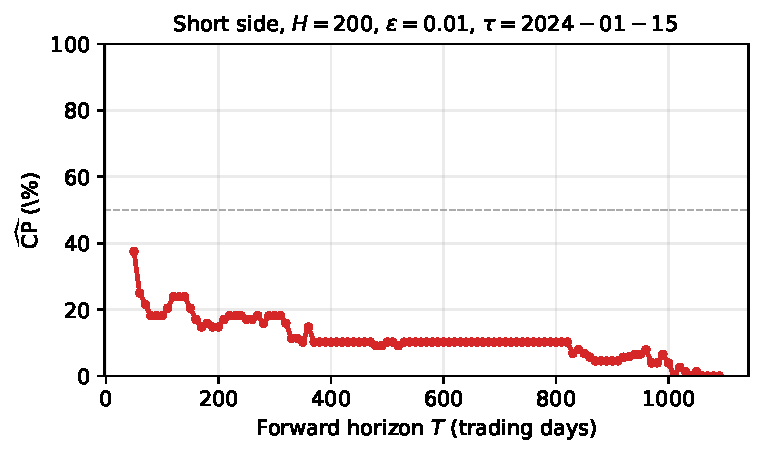
\includegraphics[width=0.92\linewidth]{cp_vs_T_20240115_H200}
  \caption{CMAPS short-side $\widehat{\CP}$ versus forward horizon $T$ with $H=200$, $\eps=0.01$, $\tauan=\text{2024-01-15}$. Points with $n<5$ are omitted.}
  \label{fig:cp-vs-t}
\end{figure}

Changing $H$ or $\eps$ shifts both $n$ and the composition of $B$; the next section treats that exploration systematically.
% <<< end sections/illustration.tex

% >>> begin sections/diagnostics.tex
\section{Parameter-surface diagnostics}
\label{sec:diagnostics}

CMAPS is used by sweeping $(H,T,\eps)$ on a discrete grid.
The analog-matching idea is classical---select past states resembling the present, then read off outcomes \cite{lorenz1969empirical}---but here the match rule is explicit and every analog is listed.

\paragraph{Heatmaps and slices.}
For fixed $\eps$, evaluate $\widehat{\CP}(H,T)$ on the configured grid (e.g.\ $H \in \{65,\ldots,1000\}$, $T \in \{90,\ldots,1095\}$).
Cells show $\widehat{\CP}$ and $n$; fixing $H$ and plotting versus $T$ (Figure~\ref{fig:cp-vs-t}) is one slice through this surface.

\paragraph{Tolerance sweep.}
Shrinking $\eps$ tightens the state match and lowers $n$; widening $\eps$ does the reverse.
A log-spaced sweep shows whether a headline $\widehat{\CP}$ is stable or an artifact of tolerance choice.

\paragraph{Ranking and reproducibility.}
Strategies rank by $\widehat{\CP}$ or $\widehat{\CP}_{\mathrm{smooth}}$, with optional minimum $n$.
The reference implementation is deterministic: the same $(\tauan,H,T,\eps)$ reproduces the same ledger, with $\sum Y_{t,T} = h$ and $|B|=n$ on golden test cases.
% <<< end sections/diagnostics.tex

% >>> begin sections/conclusion.tex
\section{Conclusion}
\label{sec:conclusion}

CMAPS estimates a directional conditional probability by matching Bitcoin's current price-to-moving-average state to historical analogs and counting forward successes over horizon $T$.
The method is deliberately simple: set arithmetic in \eqref{eq:k}--\eqref{eq:cp}, optional smoothing in \eqref{eq:smooth}, and full enumeration of contributing dates.

For quantitative analysts, the practical value is twofold.
First, $\widehat{\CP}$ is interpretable as a sample frequency with transparent $n$.
Second, $(H,T,\eps)$ diagnostics make sensitivity visible rather than hidden inside a composite indicator.

Reasonable extensions---same framework, not required for the core method---include alternative averages (EMA), explicit return summaries $\bar{R}_{t,T}$ conditional on $B$, and additional assets.
CMAPS as specified here is a self-contained building block: a formal analog-matching conditional probability for Bitcoin trend states.

\paragraph{Disclaimer.}
Historical analog frequencies are descriptive statistics.
They are not investment recommendations and do not incorporate costs, funding, or execution constraints.
% <<< end sections/conclusion.tex


\begingroup
\small
\bibliographystyle{plain}
\bibliography{references}
\endgroup

\end{document}
